\documentclass[10pt,letterpaper]{article}
\usepackage[T1]{fontenc}
\usepackage{lmodern,amsmath,amssymb,mathtools,booktabs,graphicx,microtype}
\usepackage[margin=0.89in,top=.83in,bottom=.86in]{geometry}
\usepackage{xcolor,fancyhdr,enumitem}
\usepackage[colorlinks=true,linkcolor=teal!58!black,urlcolor=teal!58!black,citecolor=teal!58!black]{hyperref}
\definecolor{ink}{HTML}{183543}
\definecolor{tealink}{HTML}{246757}
\definecolor{muted}{HTML}{526772}
\setlength{\headheight}{15pt}
\setlength{\parindent}{1.2em}
\setlength{\emergencystretch}{2.1em}
\setlist{topsep=3pt,itemsep=2pt}
\pagestyle{fancy}\fancyhf{}
\fancyhead[L]{\small\sffamily\color{muted}Intrinsic geometry of rectangular boxes}
\fancyhead[R]{\small\sffamily\color{muted}Constructive geometry}
\fancyfoot[C]{\small\sffamily\thepage}
\renewcommand{\headrulewidth}{.25pt}
\usepackage{titlesec}
\titleformat{\section}{\Large\sffamily\bfseries\color{ink}}{\thesection}{.6em}{}
\titleformat{\subsection}{\large\sffamily\bfseries\color{tealink}}{\thesubsection}{.6em}{}
\titlespacing*{\section}{0pt}{2ex plus .5ex}{.8ex}
\titlespacing*{\subsection}{0pt}{1.8ex plus .5ex}{.6ex}
\newcommand{\R}{\mathbb R}
\newcommand{\Q}{\mathbb Q}
\newcommand{\cB}{\partial B}
\newcommand{\ipra}{\textsf{iPRA}}
\newcommand{\sqnorm}[1]{\lVert #1\rVert_2^2}
\hypersetup{pdftitle={Farthest points on a rectangular N-box},pdfsubject={Intrinsic geometry and constructive arithmetic}}
\begin{document}
\thispagestyle{empty}
{\sffamily\small\color{tealink}\bfseries CONSTRUCTIVE GEOMETRY\hfill 19 NOVEMBER 2026\par}
\vspace{1em}
{\Huge\sffamily\bfseries\color{ink} Farthest points on a rectangular \(N\)-box\par}
\vspace{.45em}
{\Large\sffamily\color{muted} Vertex eccentricity, intrinsic diameter, and exact coordinates\par}
\vspace{.8em}\hrule\vspace{.8em}
Let $B=\prod_{i=1}^N[0,a_i]$, with positive side lengths and $N\ge2$.
The surface is the entire boundary, including the interiors of its $(N-1)$-dimensional facets. A path has Euclidean arc length and must stay on this boundary at all times. Denote its intrinsic distance by $d$. For a prescribed vertex $v$, the two objectives are
\[
 E=\max_{y\in\cB}d(v,y),\qquad D=\max_{p,q\in\cB}d(p,q).
\]
Reflection of each axis where $v_i=a_i$ carries $v$ to the origin. All coordinates below are in this reflected system unless stated otherwise. Undo those reflections in the reported maximizers. The side lengths can be supplied in any order.
\paragraph{General answer.}
For $E$, place each possible unfolded image of the source in each target facet chart. On each $k$-dimensional coordinate face of the chart, intersect $k$ independent perpendicular bisectors from $k+1$ images with its affine hull. Include all corners. Evaluate the true surface distance at the candidates. A candidate giving the largest value supplies $Y$ and $E=d(v,Y)$. This uses only linear solves and ordered segment tests. In particular, rational side lengths give rational maximizing coordinates and rational $E^2$.
\par For $D$, the two endpoints are independent. On the product of two facet charts enumerate the squared lengths $Q_w(p,q)$ of straight developments and their crossing tests $V_w(p,q)$. Compute the largest $h$ satisfying
\[
   h\ge0,\qquad \exists p,q\quad
         \bigwedge_w\bigl(V_w(p,q)\ \Longrightarrow\ h\le Q_w(p,q)\bigr).
\]
Take the largest result over the chart pairs. The same algebraic calculation returns coordinates $P,Q$ that realize $D=\sqrt h$. The existence test with $h>E^2$ decides exactly whether freeing the first endpoint helps. Sections~\ref{sec:free} and~\ref{sec:algebraic} give finite evaluation and witness algorithms. These are uniform answers for variable $N$ and arbitrary positive algebraic lengths. The number of polynomials grows quickly.
\paragraph{Closed results.}
Let $S=\sum_i a_i^2$ and $a_{(1)}\le\dots\le a_{(N)}$ be the sorted sides. Opposite corners have squared distance $S+2a_{(1)}a_{(2)}$. For a cube of side $a$, $E=D=a\sqrt{N+2}$. For $N\ge3$ its only diametral pairs are opposite vertices. For $[0,b]\times[0,a]^{N-1}$, $0<b\le a$, opposite vertices also attain both maxima, with squared distance $S+2ab$.
\par A long prism behaves differently. On $[0,1]^{N-1}\times[0,C]$, $C\ge1$, $N\ge3$, the winning vertex-source target changes from the opposite corner to an interior point of the top facet. Section~\ref{sec:prismfixed} gives the transition explicitly. For $C>N/2$ the unrestricted diameter strictly exceeds $E$. For $C\ge N-1$, Section~\ref{sec:freeprisms} gives $D$ and the maximizing pair in radicals. If $N\ge6$, the prism diameter has a closed formula for every $C\ge1$.
\par\smallskip
For arbitrary side lengths given by fast Cauchy approximations we compute the extremal values and endpoint witnesses to any requested error. The prism transition proves that a uniform algorithm returning one \emph{exact} maximizing point from this input representation is impossible. The finite statements used in the proofs are specified in the language of intuitionistic primitive recursive arithmetic.

\medskip
\noindent\colorbox{teal!5}{\parbox{.965\linewidth}{\small
\textbf{A four-dimensional example.} On $[0,1]^3\times[0,5]$ the vertex-source answer is $Y=(3/5,3/5,3/5,5)$, with $E^2=802/25$. Put $u=\sqrt6-2$ and $v=3-\sqrt6$. The pair $(u,u,u,0)$ and $(v,v,v,5)$ attains $D^2=134-40\sqrt6$.}}
\clearpage
\section{Dimension, charts, and the arithmetic interpretation}
We write $n=N$ interchangeably and use $d$ for the base dimension when studying prisms. In dimension two the boundary is a circle of perimeter $2(a_1+a_2)$ in arclength coordinates. The shorter of the two arcs is at most $a_1+a_2$. Exactly the pairs half a perimeter apart attain this bound. From a given corner the answer is the opposite corner. In dimension one the boundary consists of two isolated endpoints. No path joins them, so there is no finite intrinsic diameter (the extended distance is $+\infty$). If the empty product is allowed in dimension zero, its boundary in $\R^0$ is empty.
\par A chart specifies a coordinate fixed to its lower or upper bound. At a lower-dimensional face several charts are available. Exact finite inputs can be rational or real algebraic numbers. The latter are given by polynomials and root identifiers. For the accuracy version, an endpoint is a chart and normalized coordinates $u_i\in[0,1]$, represented by rationals within specified errors. Its physical coordinates are $a_i u_i$. A named positive side comes with, or can be considered at any fixed stage with evidence for, a positive rational lower bound. Upper bounds and the necessary evaluations of real names suffice for the value algorithms. Continuous paths in the usual statement may be completely arbitrary. Inside first-order arithmetic their role is expressed by finite lists of samples, a step bound and rational error bounds. No real, function-space quantifier or compactness axiom is added to iPRA.
\par The rectangular archive treats $N=3$ by a few explicit planar unfoldings; the second attachment treats skew three-dimensional cells with a Gram matrix. We use the finite face-chain idea from the latter. A high-dimensional gate is a rectangle of dimension $N-2$, and three-or-more-facet intersections require a local shortening proof. Both enter below. The finite program never imposes central symmetry on the free pair. The published three-dimensional diameter is due to Nikonorov and Nikonorova~\cite{nik}. For general polytope source unfoldings see Miller and Pak~\cite{mp}.


\section{Why finitely many facet chains suffice}
\label{sec:chain}
Write $B=\prod_{i=1}^n[0,a_i]$ and let $F_{i,b}$ denote the facet
$x_i=b$, where $b=0$ or $a_i$. A point may have several facet tags.
An admissible word $(F_1,\ldots,F_m)$ has pairwise distinct letters,
$x\in F_1$, $y\in F_m$, and nonempty consecutive intersections.
A gate $z_j$ is any point in $F_j\cap F_{j+1}$. With
$z_0=x$, $z_m=y$, the cost is
\[
                  \sum_{j=1}^{m}\|z_j-z_{j-1}\|_2.
\]
Each chord lies on the boundary by convexity of its facet. The number
of letters is at most $2n$. The gate box is closed even when a minimizing
chord has length zero or lies entirely along an intersection.

\paragraph{Compression of an arbitrary path.}
Let $\gamma$ be a boundary path from $x$ to $y$. Suppose $L$ bounds
all its sampled polygonal lengths. Pick $h>0$ with $3h<\min_i a_i$.
Use a modulus of uniform continuity to sample $x_0,\ldots,x_M$ in
time order, endpoints included, with adjacent distances at most $h$.
At each sample choose a tag whose defining coordinate has error at
most $h$. To make this a bounded arithmetic choice, approximate all
$2n$ absolute coordinate residuals to $h/4$ and minimize the rational
approximations. The actual minimum residual is zero. At the endpoints
use specified exact incident tags, available in the endpoint charts.

Starting at sample $s=0$, take $e$ to be the last sample with the
tag of $s$. Retain the block $[s,e]$ and continue at $e+1$ until the
samples end. No later block can have the tag of an earlier block.
Successive blocks have different tags $F,G$, and the gap between
them consists of one step $x_e$ to $x_{e+1}$. If $F,G$ were opposite
facets, their separation would be at most $h+h+h$, a contradiction.
Thus their axes differ. In $x_e$ set the two tagged coordinates
to the boundary values of $F$ and $G$, obtaining a gate $z$.
The two corrections are at most $h$ and $2h$ respectively, so
\[
             \|z-x_e\|_2\le 3h,\qquad
             \|z-x_{e+1}\|_2\le 4h .
\]
Take the chords joining successive gates, including the original
endpoints. Triangle inequalities show that their total cost is at most
\[
   \sum_{\text{blocks }[s,e]}\|x_s-x_e\|_2+7(2n-1)h
                     \ \le\ L+7(2n-1)h.
\]
The first terms are bounded by disjoint portions of a sampled
polygonal length. This estimate is independent of $M$. It applies even
to a curve that changes facets infinitely often in a finite interval.
The bounded scan for last occurrences uses tag equality alone.

Conversely, every coded chain is a surface path. Sending the specified
precision to zero proves that the intrinsic distance is the infimum
of costs of these finitely many gate-box problems. In ordinary real
geometry a smallest cost is attained by continuity on the finite union
of compact gate boxes; for real algebraic input the arithmetic witness
can be selected over the real algebraic numbers. The constructive
finite-precision argument needs no choice of a minimizing real point:
if every gate is rounded in its free coordinates to a boundary-respecting
grid with displacement at most $\rho$, the cost increases by at most
$2(m-1)\rho$. Thus the smallest grid cost for fixed endpoints differs
from the path distance by at most $2(2n-1)\rho$, uniformly.

\paragraph{The first-order reading.}
An ambient arbitrary continuous function is external to first-order
arithmetic. Internally use finite rational samples with a tolerance
and a length bound. The preceding argument consumes a finite sample
with the stipulated step-size bound, so its index scan, choice of tags,
coordinate replacement and chain construction are primitive recursive
in these data. For a named path supply a primitive-recursive dyadic
evaluation and a modulus (or pass the needed samples and modulus
values as inputs). Replacing the ideal samples in the triangle
inequalities by their stated dyadic enclosures and increasing the
precision gives the same conclusion at each output precision. It is
important that no error proportional to $M$ was used: block endpoints
may be compared directly with true samples, and only $2n$ such
comparisons enter the compressed length. The ordinary interpretation
for every continuous rectifiable path follows from its uniform
continuity and the definition of length as a supremum over finite
partitions.


\section{The fixed-vertex problem reduces to linear algebra}
\label{sec:fixedarr}
For rational side lengths there is a rational maximizing point, and the
square of the maximum distance is rational. This gives a smaller exact
calculation for the first problem. The construction works for any prescribed
rational source on the boundary. It uses all possible facet sequences, and
tests their visibility from the source. For algebraic data the same
calculation takes place in the ordered field generated by the input.

\subsection{Why a minimizing path unfolds to one line}
Choose a shortest polygonal path with as few genuine bends as possible,
merging collinear consecutive segments and discarding segments of length zero.
For algebraic endpoints the bounded polygonal minimization can be done over
the real algebraic numbers. All comparisons in the following local argument
then have decidable signs.
A segment contained in the boundary of a box is contained in a facet. Indeed a facet equation that holds at an interior point of a segment holds at
both endpoints, by the coordinate bounds. If two nonconsecutive pieces
can be assigned to the same facet, replace the intervening path between
interior points of those pieces by its chord. It shortens the path strictly
when there is a genuine intervening bend. Thus the facets used by distinct
pieces of a bent minimizing path are distinct.

Let $x$ be a genuine bend. Among the coordinates whose bounds are attained at
$x$, reflect upper bounds and translate so that the $k$ active inward
coordinates at $x$ are zero. Use points $A,B$ on the incident legs, both at
the same small distance $r>0$ from $x$, and take $x$ as origin. Choose $r$
small enough that inactive facets are avoided. Each point has a zero active
coordinate. If they share a zero, their chord lies in the corresponding facet
and strictly shortens the bent path. Otherwise take $A_i=0$, $B_j=0$ with
$i\ne j$. If $k\ge3$, choose another active coordinate $l$. Then
$A_l+B_l>0$. For $w=t e_l$, both $[A,w]$ and $[w,B]$ are boundary segments.
For small positive $t$, the elementary inequality
$\sqrt{r^2+s}\le r+s/(2r)$ gives
\[
 |A-w|+|B-w|
 \le 2r+\frac{t^2-t(A_l+B_l)}r <2r .
\]
Here $0<t<A_l+B_l$ and $t$ is also chosen small enough to stay in the
box. The case $k=1$ already gives a common facet. Consequently every
genuine bend lies in the relative interior of a ridge, exactly two
facets meeting there. Near the bend, laying these two facets flat makes
an open Euclidean neighborhood. The straight chord in that neighborhood
shows that the developed path is straight across the ridge. The crossing is transverse because a developed line tangent to the ridge stays in its
hyperplane and would give no bend. Successively laying the facets flat
therefore gives one straight line segment. A path with no bends lies in a
single facet. When computing on the relative interior of a target facet,
that facet is the last one. Points on its boundary will be recovered by
continuity.

\subsection{Visibility tests with a fixed source}
Write $m=N-1$ and identify a target facet with an $m$-dimensional coordinate
box $F$. Enumerate words of distinct facets ending with $F$, beginning with
a facet containing the source, and with consecutive facets sharing a ridge.
Develop each word backwards into the coordinate space of $F$. Each step
fixes the common ridge and places the new box on the opposite side of its
supporting hyperplane. Coordinate axes are permuted or reversed and
translations are sums of signed side lengths. Keep the developed source $S$
and, in path order, the developed ridge rectangles $H_1,\ldots,H_b$.
Each $H_h$ has a constant coordinate $i_h$ equal to $c_h$ and intervals
$[L_{hj},U_{hj}]$ in the other coordinates.

For a specified target $y$, intersect the parametrized segment
$S+t(y-S)$ with each $H_h$ for $0\le t\le1$. Each preimage $J_h$ is a
closed interval, a singleton, or empty. It is calculated simply by clipping
$[0,1]$ against the coordinate interval conditions. A zero direction
coordinate imposes either no restriction or an empty interval. Starting
at $t_0=0$, set $t_h=\max(t_{h-1},\min J_h)$ and require
$t_h\le\max J_h$. An empty interval fails the test. This chooses the earliest
possible ordered crossings by induction. Between two successive crossings,
the segment lies in the correct developed facet by convexity. Conversely
any straight realization gives such an ordered family. Thus the minimum
squared norm $|y-S|^2$ among words passing this test equals the actual
squared distance. Coincident crossings and overlapping unfolded boxes cause
no ambiguity. If the shortest path ends in a different facet at $y\in F$,
one may append $F$ with a zero-length final piece. If $F$ occurred earlier,
the chord to $y$ in that occurrence of $F$ is already optimal and supplies
a path ending there.

For a source vertex reflected to the origin, only words consisting of one
lower facet followed by distinct upper facets are needed on upper target
facets. Indeed, any point of a lower facet can be joined to the origin by
its chord on that facet, which strictly shortens any genuinely bent prefix.
The single lower facet itself suffices on any lower target facet. This
reduces the length of words in the fixed-vertex computation to at most
$N+1$ facets.

\subsection{Exact maximizing coordinates from source bisectors}
For each target facet, retain all developed sources of its listed words,
before applying any visibility test. Define
\[
 h(y)=d(X,y)^2-|y|^2,\qquad
 L_S(y)=|S|^2-2S\mathbin{\cdot}y.
\]
For every $y$, the continuous function $h$ has one of the finitely many
values $L_S(y)$. It is unnecessary to regard every developed source as a
valid competitor at $y$. Visibility is tested whenever an actual distance
is evaluated.

Cut the interior of the target box by the planes $L_S=L_T$ for distinct
affine forms. On each open cell, $h$ agrees throughout with one particular
form. Here is a finite proof of this assertion. On a segment joining any two
points of the cell, the gaps between distinct forms are at least their
smaller endpoint gaps. This follows from affinity and their unchanging order.
If there is just one form the assertion is immediate. Otherwise take the
least such positive gap $g$. Within a facet $|d(X,y)-d(X,z)|\le |y-z|$
because its chords are on the boundary. The distance is bounded, so $h$
and the finitely many forms all have explicit Lipschitz bounds there. For
instance a common bound for $h$ is $2\sup d+2\sup |y|$, and $2|S|$ bounds
the Lipschitz constant for $L_S$. Subdivide the segment until each function
changes by less than $g/3$ per step. If $h$ equals a form at one mesh
point it must equal that same form at the next, since otherwise the two distinct
form values at the next mesh point would differ by less than $2g/3$.
Finite induction proves the assertion. Continuity now gives
$d(X,y)^2=|y-S|^2$ on the closure of the cell, including all ties at
the walls.

Each closure is a bounded polytope, and the convex quadratic there takes
a largest value at a vertex. To see this last point constructively, at a
point whose tight normals have rank less than $m$, choose a nonzero vector
annihilated by them. Extend its line in each direction to the first new tight
inequality. The endpoints exist by boundedness, the rank increases, and the
original point is their convex combination. Repeat at most $m$ times per
branch. Convexity bounds the value by the greatest of the final vertex
values. To see that the closures cover the box, choose an interior point off all
listed planes and approach a proposed boundary point from it along a segment. Every plane has a constant sign on a sufficiently short terminal
part of the segment, apart from its endpoint. For a finite choice of the
interior point one may try $z_0+\epsilon(t,t^2,\ldots,t^m)$ in a small
interior box, using more than $m$ times the number of planes distinct
rational $t$ in $(0,1)$. A proper affine plane gives a nonzero polynomial
of degree at most $m$. This argument proves attainment constructively over
the real algebraic numbers. All vertices arise from $m$ independent
bisectors and facet walls. Trying those intersections inside the target
box, evaluating actual distances by the ordered gate test, and taking the
largest value already solves the problem.

There is a smaller list. For each coordinate face $G$ of a target facet
write $k=\dim G$. If $k=0$, include its vertex. Otherwise choose
$k+1$ images $S_0,\ldots,S_k$ and solve
\[
 y\in\operatorname{aff}G,\qquad
       |y-S_0|^2=|y-S_j|^2\quad(1\le j\le k).
\]
Keep the solution if the restricted system has full rank and $y\in G$.
To verify completeness, let $y$ be an attained maximum, in the relative
interior of its smallest face $G$. Collect all images whose squared norms
at $y$ equal the actual distance squared, even if some of their words fail
visibility. If the differences from one such form have rank less than $k$
on $G$, choose a nonzero tangent vector $v$ annihilated by these differences.
The tied forms stay equal along $y+tv$. All other forms stay apart from
$h$ for small $|t|$ by the finite gap and continuity. Thus on both sides of
$y$ the squared distance must be the same quadratic $|y+tv-S_0|^2$.
Its two values at $\pm t$ average to $|y-S_0|^2+t^2|v|^2$, contradicting
maximality. Full rank follows, and a subset of $k$ independent equations
places the maximizing point on the claimed list. Extraneous candidate points
do no harm because the gate test evaluates their true distance.

For rational data all sources and bisector coefficients are rational.
Cramer's rule therefore gives a rational maximizing point and rational
squared eccentricity. More generally the operations take place in the
ordered field generated by the side lengths and the fixed source
coordinates. With decidable signs the coordinates are selected from a
finite list of rational functions of these inputs. The distance is the
nonnegative square root of the selected squared value. This rationality is
specific to a fixed source. Moving both endpoints introduces variable
products. The word bounds, subset enumerations, determinant computations,
and clipping loops above all have primitive-recursive bounds on finite
codes.


\section{Exact length and coordinates when both endpoints are free}\label{sec:free}
Fix two closed facet charts and let $u,v$ list the $N-1$ free coordinates of their points. Write $p(u),q(v)$ for their ambient embeddings. For every simple word $w$ joining the charts develop the whole word in the chart of $q$. The image $s_w(u)$ is affine in $u$ with a signed permutation as its linear part. Its translation is a signed sum of side lengths. Consequently
\[
                 Q_w(u,v)=\|v-s_w(u)\|^2
\]
is a polynomial of total degree at most two. For an explicit implementation of an unfolding, a chart slot reads $o+\sigma x_j$, $\sigma\in\{-1,1\}$. Suppose the old fixed axis $i$ has side bit $\alpha$ and the new fixed axis $j$ has bit $\beta$. At the gate the slot reads $c=o+\sigma\beta a_j$. In the new facet it reads
\[
      c+\sigma(2\beta-1)(1-2\alpha)(x_i-\alpha a_i).
\]
This fixes the gate and places the two interiors on opposite sides of it. All other slots are carried through unchanged. It constructs every $s_w$ and every closed gate box.
\paragraph{A polynomial crossing test.}
On the segment $v+t(s_w-v)$ take the gates in order from $q$ toward $p$. The interval requirements for gate $j$, including $0\le t_j\le1$, are a list of rows $A t_j+B\ge0$. Their coefficients are affine expressions in the endpoint variables. A zero slope requires $B\ge0$. A positive slope is a lower bound, a negative one an upper bound. For every lower row $(A,B)$ of gate $j$ and every upper row $(C,F)$ of gate $k\ge j$, require
\[
      (A>0\ \wedge\ C<0)\ \Longrightarrow\ AF-BC\ge0.
\]
The test compares $-B/A$ to $-F/C$ with the correct denominator signs. Necessity follows from $t_j\le t_k$. For sufficiency take at each gate the largest of the preceding and current lower bounds; it is within every current upper bound. This gives the predicate $V_w$ by signs of polynomials of degree at most two. Ordered times may coincide. In particular an endpoint in several facets can attach an incident chart by a zero-length piece. If that chart occurs farther along a shortest path, the whole prefix through its last point can be replaced by its chord; the same holds for the other endpoint and the suffix. With a common chart the single chord suffices. This supplies a simple straight development for every prescribed chart pair. Alternatively, approach edge endpoints from their chart interiors. The finite list of legal segments is closed under such limits, since the crossing times lie in a closed bounded ordered simplex. The preceding chord argument avoids any need to extract a subsequence.
\paragraph{Quantifying both endpoints.}
On the closed chart boxes $U,V$ the exact condition $d(p(u),q(v))^2\ge h$ is
\begin{equation}\label{eq:win}
 (u,v)\in U\times V\quad\wedge\quad
    \bigwedge_w(\neg V_w(u,v)\,\vee\,Q_w(u,v)\ge h).
\end{equation}
At least one minimum-length word passes its test, and every passing word is a legal surface path. Thus a long developed chord that misses a gate cannot falsify~\eqref{eq:win}. Eliminate $u,v$ from~\eqref{eq:win}. Isolate the rightmost feasible $h\ge0$ on the real line. With this $h$ fixed, sample a satisfying tuple of~\eqref{eq:win}. Its chart embeddings are the promised coordinates. Do this for each chart pair and keep the largest $h$. Exact coordinates can be given as isolating roots; direct radicals are unnecessary. Existence and exact sampling over algebraic input follow from Section~\ref{sec:algebraic}. For arbitrary real parameters this same finite system describes the answer and all maximizing pairs, with roots and branch signs relative to the ordered input field.
\par A same-facet pair has squared distance at most $S-\min a_i^2$, strictly below the opposite-corner value. Independent coordinate reflections let one use just two different lower axes, or opposite sides of the same axis. Swapping the endpoints reverses the word. These reductions preserve all attainable values. For every box,
\begin{equation}\label{eq:sandwich}
   S+2a_{(1)}a_{(2)}\ \le E^2\le D^2\ \le S+2a_{(N-1)}a_{(N)}.
\end{equation}
For the upper estimate use the two-facet path for different axes; for opposite $i$-facets use a transverse $j$-face with the smaller total detour. Its perpendicular travel is at most $a_i+a_j$. The other differences are bounded by their side lengths. The constructions and the lower estimate are proved in Section~\ref{sec:families}.
\paragraph{A second exact algorithm using fewer input polynomials.}
The supplied Python reference program projects the facet walls and $Q_w-h$, with $h$ as the first variable in a cylindrical algebraic decomposition. It can omit the visibility inequalities from the projection. To justify this, on each connected sign-invariant cell inside the chart domain the continuous function $f=d^2-h$ agrees at each point with one of the $Q_w-h$. Its sign is constant. At a point where $f=0$, the finitely many nonzero candidates have a positive gap and remain separated from $f$ locally. All candidates zero there vanish on that cell. The zero set of $f$ is therefore both relatively open and closed, and off it the sign follows by continuity. One sample per cell, checked by the actual gate test, identifies the graph $f=0$. A finite endpoint of its projected range is a section (point cell) on the $h$-axis. Lift from these point cells in decreasing order to find the largest feasible height and a witnessing pair. Starting with the known opposite-corner pair permits skipping heights at or below it.
\par For clarity the reference uses the full projection: coefficients, and principal subresultants for possible leading truncations of a polynomial and its derivative, and for each pair of truncations. Specializations with all coefficients zero are handled in the lifting step. On a base cell the coefficients fix the degree; subresultant ranks fix the number of distinct roots and the degree of each pairwise gcd. Roots can then be continued in order without separating a common root or creating a collision. Locally this follows by isolating the distinct complex roots in disjoint disks: constant degree and distinct-root count force one distinct root of unchanged multiplicity in each disk, and constant pairwise gcd degree precludes a common root splitting there. Thus the real roots form ordered sections and the complementary intervals are sectors. This is the full sign-invariant projection and lifting construction~\cite{cad}. The signed-remainder elimination below supplies a wholly arithmetic alternative to this implementation. Full projection is expensive even when the final answer is short.


\section{Exact families and a strict comparison in every dimension}
\label{sec:families}
For two points $x,y$ on facets with different fixed coordinates
$i,j$, a route in just these facets has squared length
\begin{equation}\label{eq:twofacet}
       (|x_i-y_i|+|x_j-y_j|)^2+
                       \sum_{k\ne i,j}(x_k-y_k)^2 .
\end{equation}
Indeed the two distances perpendicular to the common gate are
$|x_j-y_j|$ and $|x_i-y_i|$. Unfold them into two intervals on one
line, and linearly interpolate the other coordinates in proportion
to the traveled distance on that line. All interpolants belong to
their coordinate intervals. If both perpendicular distances vanish,
the straight segment lies in the gate. For opposite $i$-facets,
the same argument in three successive slabs, via side $x_j=b$, gives
squared length
\begin{equation}\label{eq:threefacet}
        (a_i+|x_j-b|+|y_j-b|)^2+
                     \sum_{k\ne i,j}(x_k-y_k)^2 .
\end{equation}
The slabs have the common free directions $k\ne i,j$, and the
perpendicular coordinate travels their three indicated widths in order.

\paragraph{Opposite vertices.}
Put $S=\sum_k a_k^2$. The antipodal vertices have distance
\[
                  \sqrt{S+2\min_{i\ne j}a_i a_j}.
\]
In an admissible word from $0$ to $(a_1,\ldots,a_n)$ there is a
transition from a lower $i$-facet to an upper $j$-facet. Its gate
has coordinates $z_i=0$, $z_j=a_j$. Replacing the portions before
and after that gate by chords stays on these two facets. Their
optimum length is \eqref{eq:twofacet}, and every choice $i\ne j$
can be used. For $k\ne i,j$ an optimal gate has
$z_k=a_j a_k/(a_i+a_j)$.

\paragraph{The hypercube.}
For $a_1=\cdots=a_n=a$ the eccentricity of a vertex and the
unrestricted diameter both equal $a\sqrt{n+2}$ and opposite
vertices attain them. In fact a common facet gives a chord of
length at most $a\sqrt{n-1}$. For different nonopposite facets,
\eqref{eq:twofacet} is at most $(4+n-2)a^2$. For opposite
facets select either side of a transverse axis $j$ in
\eqref{eq:threefacet}; the smaller of $x_j+y_j$ and
$2a-x_j-y_j$ is at most $a$. This gives the very same bound.
The antipodal-vertex formula gives equality. For $n\ge3$ one can
also read off all equality cases. With differently indexed endpoint
facets, equality in the upper bound forces every coordinate
difference to have magnitude $a$. With opposite $i$-facets, the
same upper bound holds for every choice of transverse index $j$.
For any $k\ne i$, choose $j\notin\{i,k\}$. Equality forces
$|x_k-y_k|=a$ in that bound, since its squared contribution is
at most $a^2$. The $i$th coordinate already has full difference.
Thus all diametral pairs for $n\ge3$ are opposite vertices; the
opposite vertex is the unique farthest point from a given corner.
In $n=2$ the boundary is a polygonal loop, and every point has a
unique partner at half the perimeter.

\paragraph{Opposite cap centers.}
In $[0,1]^d\times[0,C]$, $d\ge2$, let $c=(1/2,\ldots,1/2)$. The two cap centers $(c,0)$ and $(c,C)$ have distance $C+1$. In a simple word from center to center the two caps are the first and last facets. Reaching their rims costs at least $1/2$ at each end, and the vertical displacement between the rims is $C$. Crossing to a nearest wall, moving up it, and returning to the other center attains this bound.

\paragraph{One short side, all others equal.}
Scale the long sides to one and let the thickness be $0<h\le1$.
Then $D=E=\sqrt{n-1+h^2+2h}$ for every $n\ge2$.
The opposing-vertices lower bound is already known. For the upper
bound, a common facet allows its chord. On opposite facets, cross
via one of the two faces of a transverse axis chosen to give a pair
of side lengths $1,h$, and use \eqref{eq:threefacet}. For distinct
axes including the thickness axis, \eqref{eq:twofacet} suffices.
This leaves two different lateral facets. Reflect their axes $i,j$
so that both are lower facets. Write
$u=y_i$, $v=x_j$, and $K=\sum_{k\notin\{i,j,\mathrm{thickness}\}}
(x_k-y_k)^2\le n-3$. If $uv\le h$, the two-face cost squared
is at most $u^2+v^2+2h+h^2+K$, giving the bound.

For $uv>h$ consider crossing either thickness facet (an end plate)
between the two lateral facets. Let $t,s$ be the distances of the
first and second endpoints to this plate. Develop the three facets
into the plate's hyperplane. The two relevant coordinates of the
endpoints are $(-t,v)$ and $(u,-s)$. As $ts\le h^2\le h<uv$,
the segment reaches the line $i=0$ before leaving through the line
$j=0$: its crossing fractions are $t/(u+t)$ and $v/(v+s)$.
During each of the three subsegments its remaining coordinates
stay in their prescribed intervals by linear interpolation. The
squared length is $(u+t)^2+(v+s)^2+K$.
For the other plate replace $(t,s)$ by $(h-t,h-s)$. Averaging the
two squared lengths gives at most
\[
 u^2+v^2+h(u+v)+h^2+K\le 2+2h+h^2+K,
\]
since $r^2+(h-r)^2\le h^2$ for $0\le r\le h$. One of the two
costs obeys the desired upper bound. For named real data the case
comparisons here can be used on rational approximations and the
result transported by continuity.


\subsection{Closed fixed-vertex solution for a prism with a cubical base}
\label{sec:prismfixed}
Let $[0,1]^d\times[0,C]$ have $d=N-1\ge2$ and $C\ge1$.
Write $t=(C+1)/(2C)$. The two candidate farthest points from the
origin and their squared distances are
\[
 \begin{array}{c|c}
   (1,\ldots,1,C)& L^2=C^2+d+2\\
   (t,\ldots,t,C)& R^2=C^2+d t^2+2Ct .
 \end{array}
\]
The larger value wins. The explicit difference is
\[
 R^2-L^2=\frac{(C-1)(4C^2-3dC-d)}{4C^2}.
\]
Consequently the preferred point changes at
$C=(3d+\sqrt{9d^2+16d})/8$, with a tie at that value.
For the four-dimensional $1\times1\times1\times5$ prism the off-vertex
point is $(3/5,3/5,3/5,5)$ and $E=\sqrt{802}/5$.

\paragraph{All distances on the top cap.}
For $p\in[0,1]^d$, put $m=\min p_i$, $M=\max p_i$. We prove
\[
 d(0,(p,C))^2=C^2+\sum_i p_i^2+
       \min\{2Cm,\ 2C+2-2(C+1)M+2m\}.                 \tag{P}
\]
In the chart of this cap, consider the $d$ direct images $-C e_i$
and the $d(d-1)$ images $(C+1)e_i-e_j$ for $i\ne j$.
The least squared distance to their union is the right side of (P).
For the second group one may use $p_i=M,p_j=m$. When
$M=m$ any distinct $i,j$ work.

To check completeness, develop a shortest word backwards as above. It
starts in the top cap, visits $r$ distinct upper transverse facets
$i_1,\ldots,i_r$, and ends in a lower facet. When $r=0$ the image is direct.
After $r\ge1$ upper transitions, chart slot $i_1$ reads $1+C-z$ where $z$
is height. Slot $i_k$ for $2\le k\le r$ reads $2-x_{i_{k-1}}$, and every
untouched slot reads its original coordinate. For the induction step, about the upper wall of the next unused axis the previous upper normal
coordinate is reflected, with the two unit side widths summing to $2$. On the first step those widths are $1$ and $C$. The current normal is
$i_r$. The one last transition into the initial lower facet has the
following possibilities when evaluated at the origin.
\begin{itemize}
\item If the lower axis $j$ is untouched and transverse, its slot becomes
$-1$, slot $i_1$ becomes $1+C$, and earlier folded transverse slots $i_2,
\ldots,i_r$ become $2$.
\item If the lower axis is height, slot $i_1$ becomes $C+2$ and the
other folded slots become $2$.
\item If the lower axis is $i_k$, $k<r$, slot $i_{k+1}$ becomes $3$,
slot $i_1$ becomes $1+C$, and the other folded slots become $2$.
\end{itemize}
In the first case, one verifies the new slot by writing it as
$x_{i_r}-1$. The second and third cases instead give $C+2-x_{i_r}$ and
$3-x_{i_r}$ respectively. In every case the unmentioned untouched slots are zero.
These are all possibilities, since opposite facets of the current normal
cannot be adjacent.

For $0\le u\le1$, replacing a $2$ by $0$ or a $3$ by $-1$ weakly
decreases squared distance to $u$. The first and third cases are therefore
dominated by an image $(C+1)e_i-e_j$. In the second, first replace
the $2$'s by zeros. Replacing $C+2$ by $C+1$ saves
$2C+3-2p_{i_1}\ge2C+1$. Replacing a zero in any other slot by $-1$
costs $1+2p_j\le3$. Since $C\ge1$ the total distance again weakly
decreases. Hence the right side of (P) bounds the squared distance below.

Direct images are valid throughout the cap. Suppose a shortest image
is of the form $(C+1)e_i-e_j$. Comparing it with the direct image
$-C e_j$ gives $(C+1)p_i+(C-1)p_j\ge C+1$, so $p_i+C p_j\ge1$.
In the two relevant chart coordinates its segment runs from
$(C+1,-1)$ to $(p_i,p_j)$. It crosses $x_j=0$ at time
$1/(1+p_j)$ and $x_i=1$ at time $C/(C+1-p_i)$. The former occurs first
precisely when $p_i+C p_j\ge1$. At the first gate $1\le x_i\le1+C$,
and at the second $0\le x_j\le1$. All remaining coordinates interpolate
between $0$ and $p_k$ inside their allowed intervals. The ordered gates
give a valid path through the lower $j$-facet, upper $i$-facet, and
upper cap. This proves (P) also at degeneracies by the weak inequalities.

\paragraph{Optimizing the cap.}
For fixed $m,M$, $\sum p_i^2\le m^2+(d-1)M^2$, attained with only one
coordinate equal to $m$ and all others $M$. Over the triangle
$0\le m\le M\le1$, the two branches in (P) meet on
$(C-1)m+(C+1)M=C+1$. Each branch is a convex quadratic on its own
polygon. The only vertices to inspect are $(0,0),(0,1),(1,1),(t,t)$,
also allowing coincidences when $C=1$. The two $m=0$ points give
at most $C^2+d-1$. The two remaining values are $L^2$ and $R^2$ above.
On a lower facet a chord suffices and has squared length at most
$C^2+d$. On an upper transverse facet one can unfold it against a
lower transverse facet of a different axis, since $d\ge2$. The two-facet
squared length is bounded by $4+(d-2)+C^2=L^2$. This establishes the
claimed maximum over the entire surface.

In particular, permitting a free first endpoint gives a strict gain for
every $C>(d+1)/2=N/2$. The cap-center pair has distance $C+1$.
Now $(C+1)^2-L^2=2C-d-1>0$, and
\[
  4C^2\big((C+1)^2-R^2\big)=4C^3-d(C+1)^2
       >4C^3-(2C-1)(C+1)^2=(C-1)^2(2C+1)\ge0.
\]
The general algorithm decides the comparison for the remaining algebraic inputs.


\begin{figure}[htbp]
\centering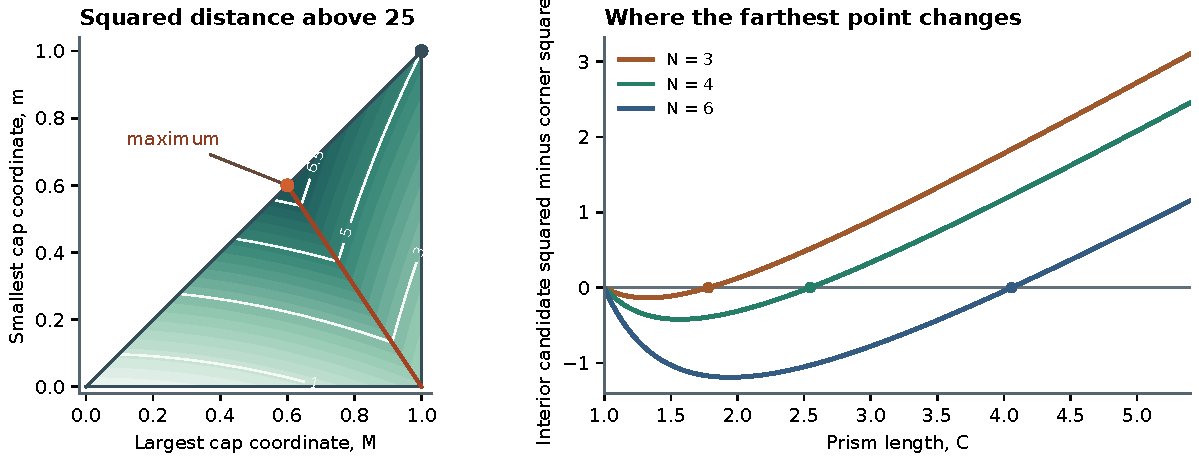
\includegraphics[width=.95\linewidth]{prism_figure.pdf}
\caption{At left, take $N=4$ and $C=5$. For prescribed smallest and largest cap coordinates $m,M$, the contours give the greatest squared distance from the origin minus $25$. The two quadratic pieces meet along the orange segment. The maximum lies at $(M,m)=(3/5,3/5)$. At right, the sign of $R^2-L^2$ determines whether the interior point or the opposite corner is farther.}
\end{figure}


\section{Exact unrestricted diameter of long prisms with cubical base}
\label{sec:freeprisms}
For $B=[0,1]^d\times[0,T]$ with $d=N-1\ge2$ and
$T\ge d$, put
\[
 \delta=\frac{T-\sqrt{T^2-1}}2
       =\frac{1}{2(T+\sqrt{T^2-1})}.
\]
Then an unrestricted maximizing pair is
\[
 ((\tfrac12-\delta)\mathbf{1},0),\quad
 ((\tfrac12+\delta)\mathbf{1},T),\qquad
 D^2=(T+1)^2+4(d-1)\delta^2.
\]
Here $\mathbf{1}$ has $d$ coordinates. The result in particular shows that
the cap centers can be strictly improved, however long the prism is.
The displayed threshold is sufficient; the argument does not locate the
first aspect ratio at which these points maximize.

\paragraph{Reduction to opposite cap interiors.}
Two lateral points can be joined by lifting a path on the base boundary,
varying height in proportion to base arclength. A vertical segment suffices
if the base coordinates coincide. This yields a length at most
$\sqrt{T^2+d+2}<T+1$, since $T\ge d\ge2$. Two points on a common cap
admit a chord of length at most $\sqrt d<T+1$.

Now let one endpoint lie on a lateral wall and the other be in a cap
at distance $u$ from its nearest rim. Projecting to that rim and lifting
as above gives length at most $\sqrt{T^2+d+2}+u$. A second route
unfolds the endpoint's lateral wall directly with the cap. All horizontal
coordinates of the cap point lie in $[u,1-u]$. Its distance to the wall
is therefore at most $1-u$, and the remaining $d-1$ coordinate differences
are each at most $1-u$. The second route thus costs at most
$\sqrt{(T+1-u)^2+(d-1)(1-u)^2}$.
Set $u_0=d/[3(d+2)]$ and $w=1-u_0$. For $u\le u_0$ the first bound is
strictly less than $T+1$, because $d+2<2dw+w^2\le2Tw+w^2$.
For $u\ge u_0$ the second is strictly less than $T+1$, because
$dw^2<1+2du_0\le1+2Tu_0$. For an explicit check of the two strict
inequalities, multiply the two positive differences by $9(d+2)^2$.
Writing $h=d-2\ge0$ gives respectively
$3h^3+28h^2+64h+4$ and $2h^3+9h^2+12h+40$.
The cap centers are at distance $T+1$, leaving only opposite cap interiors.

\paragraph{Upper bound using at most two lateral walls.}
Let the bottom and top horizontal coordinates be $p,q$. Reflect each
axis as needed to arrange $p_i\le q_i$. Write $r_i=(q_i-p_i)/2$,
$m_i=(q_i+p_i)/2$. Let $x\ge y$ be the two largest $r_i$, attained
on axes $j,k$. The route along the better of the two walls on the axis
of $x$ has squared length at most
\[
 U(y)=(T+1)^2+4(d-1)y^2.
\]
Indeed the smaller sum of depths of the two endpoints from these two
walls is at most one, and the remaining differences are at most $2y$.

Consider also the development through the lower wall on axis $j$ and
the upper wall on axis $k$, ordered from bottom to top. Set
$a=p_j$, $b=q_j$, $u=1-q_k$, $v=1-p_k$ and
$K=4\sum_{l\ne j,k}r_l^2$. Its squared straight distance is
\[
 W=(T+a+u)^2+(b+v)^2+K.
\]
In the top chart the image of $p$ has coordinates $T+1+a$ in slot
$k$ and $-v$ in slot $j$. Moving from $q$ to this image, the gate
fractions are $u/(T+a+u),\ b/(b+v),\ (T+u)/(T+a+u)$.
The denominators are positive in the cap interiors. Ordered crossings
are therefore equivalent to $uv\le b(T+a)$ and $ab\le v(T+u)$.
The other coordinates interpolate within the box. Even if a gate order
fails, $W$ is an upper bound on squared intrinsic distance. If the
first inequality fails, $b<u$ because $T+a\ge v$, and the single lower $j$-wall route has squared
cost minus $W$ equal to
$2[(T+a)(b-u)-v(u+b)]<0$. If the second fails, $v<a$ because $T+u\ge b$, and the single upper
$k$-wall route gives $2[(T+u)(v-a)-b(v+a)]<0$.

Swap the roles of $j,k$ if necessary so that $e=m_j-m_k\le0$.
The first two components of $W$ are the squares of the nonnegative
numbers $T+1-x-y+e$ and $1+x+y+e$. Omitting $e$ can only increase
them. Also $K\le4(d-2)y^2$. At fixed $y$, the sum
$(T+1-s)^2+(1+s)^2$ decreases for $s=x+y\in[2y,1]$ because
$T\ge2$; subtracting the values at $s_2\ge s_1$ gives
$2(s_2-s_1)(s_2+s_1-T)\le0$. Thus
\[
 d((p,0),(q,T))^2\le \min\{U(y),V(y)\},\quad
 V(y)=(T+1)^2+1-4Ty+4dy^2.
\]
The function $U$ increases, and $V$ decreases on $[0,1/2]$ because
$T\ge d$. The difference $V-U=1-4Ty+4y^2$ changes sign exactly
at $\delta$ in this interval. The common value $U(\delta)$ bounds
all opposite-cap distances squared.

\paragraph{Lower bound on every competing word.}
Use the displayed symmetric pair. It satisfies $0<\delta<1/6$
(as $T>5/3$). In any simple word let $F,G$ be respectively the first
and last lateral walls, regarded as facets of the base cube $C=[0,1]^d$.
Project the first cap leg orthogonally onto $F$, the last onto $G$,
and all lateral legs onto $\partial C$ by forgetting height.
The resulting base boundary path, of length $H$, goes from $P$, the
projection of $p$ onto $F$, to $Q$, the projection of $q$ onto $G$.
For each original leg its length is the Euclidean norm of two numbers:
projected length and absolute displacement in the omitted direction.
The sum of the latter numbers is at least
$T+\mathrm{dist}(p,F)+\mathrm{dist}(q,G)$.
The two-dimensional triangle inequality gives, for word cost $L$,
\[
 L^2\ge H^2+
 [T+\mathrm{dist}(p,F)+\mathrm{dist}(q,G)]^2.
\]
If the two cap depths sum to at least one, then $H^2\ge4(d-1)\delta^2$.
Indeed the $d-1$ transverse coordinates have differences $2\delta$
for parallel walls. For differently indexed walls, the two distinguished
coordinate differences are at least $1/2-\delta\ge2\delta$, and all
other differences equal $2\delta$. This case gives $L^2\ge U(\delta)$.

Otherwise $F$ is a lower wall and $G$ an upper wall, and the depth sum
is $1-2\delta$. We prove
\[
 H^2\ge(1+2\delta)^2+4(d-2)\delta^2.                 \tag{*}
\]
Whenever a base path hits a wall on coordinate $l$ at value $b$,
reflect its portion after that hit in the wall plane. The chord of
the reflected path gives a lower bound with coordinate $l$ replaced
by $|P_l-b|+|Q_l-b|$ and all other coordinate differences retained.
If $F,G$ are opposite walls on the same axis, the base path must
hit a transverse wall. Reflection there gives
$H^2\ge2+4(d-2)\delta^2$, which implies $(*)$.

For different axes, a path contained in $F\cup G$ must meet the
common ridge. Straightening the two parts inside their facets and
unfolding gives $(*)$, since the two perpendicular distances add
to $1+2\delta$. If the path hits any third wall $J$ opposite to
$F$ or $G$, its reflected coordinate has magnitude $3/2-\delta
\ge1+2\delta$ and the $d-2$ remaining transverse differences are
retained. If $J$ is on a third axis, reflection there instead gives
\[
 H^2\ge1+2(1/2+\delta)^2+4(d-3)\delta^2 .
\]
The excess over the right side of $(*)$ is
$1/2-2\delta-6\delta^2\ge0$ for $0\le\delta\le1/6$.
These alternatives exhaust the projected polygonal paths, also when
they follow a ridge or meet several walls simultaneously. In this
last depth case the resulting bound is
\[
 L^2\ge (T+1-2\delta)^2+(1+2\delta)^2+4(d-2)\delta^2
       =V(\delta)=U(\delta).
\]
A single-wall unfolded route has exactly this common squared length.
The finite-chain theorem transfers the lower bound to all surface paths,
completing the proof. For $d=3,T=5$ it gives
$D^2=36+2(5-2\sqrt6)^2=134-40\sqrt6$.


\subsection{All aspect ratios in base dimension five and higher}
For $d\ge5$ and every $T\ge1$, the unrestricted squared diameter is exactly
\[
 \max\{L_0^2,U(\delta)\},\qquad L_0^2=T^2+d+2 .
\]
Whenever the first entry wins, opposite vertices attain it. Whenever the
second entry wins, the cap pair of Section~\ref{sec:freeprisms} attains it. Freeing the source gives a
strict improvement exactly when $U(\delta)>L_0^2$. Indeed, if the
fixed-source interior point beats $L_0$, the fixed-source formula gives
$d<4T^2/(3T+1)$, whence $dt^2<(T+1)^2/(3T+1)<T$, and consequently
$E<T+1$. Writing $z=T-\sqrt{T^2-1}=2\delta$, the sign of
$U(\delta)-L_0^2$ is the sign of
\[
 (z-1)\big[(d-1)z^2+dz-1\big],
\]
because this product is $z[U(\delta)-L_0^2]$. Thus the strict regime
is $z<2/(d+\sqrt{d^2+4d-4})$.

First suppose $T\ge2$. The proof above for the opposite-cap upper bound only used $T\ge2$
until comparing $U$ and $V$. On $[0,\delta]$ the minimum is at most
$U(\delta)$; on $[\delta,1/2]$ the convex quadratic $V$ is bounded by
$\max(V(\delta),V(1/2))=\max(U(\delta),L_0^2)$. The proof of the
matching cap-pair lower bound used only $\delta\le1/6$, true for
$T\ge2$.

For $1\le T\le2$ return to the two-wall upper bound before setting
$x=y$. It is
$(T+1-x-y)^2+(1+x+y)^2+4(d-2)y^2$, a convex quadratic on
$0\le y\le x\le1/2$. At its three vertices the respective values are
$T^2+2T+2$, $T^2+T+5/2$, and $T^2+d+2$. Each is at most $L_0^2$
since $2T\le d$. The opposite corners realize $L_0$. Here
$z\ge2-\sqrt3>1/5$ and $d\ge5$, so $(d-1)z^2+dz-1>0$ and
$U(\delta)\le L_0^2$ as claimed. At $T=1$ the two entries agree
and the displayed cap pair itself consists of opposite corners.

The common-cap and lateral--lateral bounds are immediate.
For the remaining lateral-to-cap case we prove the uniform estimate
$\max(L_0,T+1)$.

As above let $u$ be the end-cap point's distance to its nearest rim, and
let $r$ be the corresponding point on that rim, on base facet $k$.
All $r_l$, $l\ne k$, lie in $[u,1-u]$. Write $P$ for the given lateral
point's projection into the unit base boundary. A base route from $P$
to $r$ has squared length at most
\[
 H(u)=\max\{4+(d-2)(1-2u)^2,\ (2-u)^2+(d-2)(1-u)^2\}.
\]
In fact for different-axis base facets the ordinary two-facet route
has total perpendicular distance at most $2-u$, with the other
differences at most $1-u$. A common facet allows the chord. For
opposite $k$-facets take any $j\ne k$ maximizing
$w=|P_j-r_j|\le1-u$. The cheaper $j$-wall detour has transverse
developed component $2-|1-P_j-r_j|$, which is at most
$2-\max(0,w-(1-2u))$ by $|1-2r_j|\le1-2u$ and the triangle
inequality. Its remaining sum of squares is at most $(d-2)w^2$.
This bound increases up to $w=1-2u$ on the first interval and is
convex from there to $w=1-u$. The two possible outer values give $H$.

The two routes give the following length bound.
\[
  \min\left\{u+\sqrt{T^2+H(u)},       \sqrt{(T+1-u)^2+(d-1)(1-u)^2}\right\}.
\]
It suffices to compare at
$T_0=(d+1)/2$, where $L_0=T_0+1$. For the rim route its excess over
$L_0$ increases with $T$ below $T_0$ since $H(u)\le d+2$, while its
excess over $T+1$ decreases above $T_0$. These monotonicities follow
by rationalizing differences of square roots (or comparing their slopes).
For the direct route the difference of squared values against $L_0^2$
increases with $T$ and against $(T+1)^2$ decreases with $T$.

At $T_0$ the rim bound holds exactly when
\[
 (4d-9)u^2+(11-3d)u\le0,\qquad
 (d-2)u^2+(3-d)u\le0,
\]
by expanding the two terms of $H(u)$ and squaring. If $d\ge7$ both
hold for every $u\in[0,1/2]$. In dimensions $d=5,6$ they hold for
$u\le1/3$. For $u\ge1/3$ the direct route suffices in those two
dimensions, since $d(1-u)^2\le1+(d+1)u$ there, as is checked at
$u=1/3$. This proves the remaining upper bound.


\paragraph{Why arbitrary Cauchy input gives approximate endpoint witnesses.}
The prism transition exhibits a genuine obstruction to uniform exact
selection. Write $C_*=(3d+\sqrt{9d^2+16d})/8>1$. On each open
branch near $C_*$, its winning point is the unique maximizer.
Indeed both cap quadratics are strictly convex in $(m,M)$, with
positive diagonal quadratic coefficients $1$ and $d-1$; a
nonvertex convex combination cannot realize the largest vertex
value. Only the displayed winning vertex of the partition does so,
and $m=M$ fixes all coordinates. On a lower facet the chord bound
is strict. On an upper transverse facet $i$, unfolding via lower
transverse facet $j\ne i$ bounds the square by
$(1+p_j)^2+\sum_{k\ne i,j}p_k^2+z^2$. Equality with
$C^2+d+2$ forces all transverse coordinates to be one and $z=C$.
Thus the one-sided limiting maximizers at $C_*$ differ in each
transverse coordinate by $1-(C_*+1)/(2C_*)>0$.

An algorithm that reads arbitrary fast Cauchy names, and returns a
name for an exact maximizing point, must provide one transverse
coordinate to an accuracy less than a quarter of this gap after
finitely many input queries. Run it on a name of $C_*$ whose
rational responses lie strictly inside all required error bounds.
Those same finitely many responses are compatible with names of
numbers on either side as close to $C_*$ as desired. The algorithm
gives the same coordinate approximation for both, contradicting
the separated unique outputs. This already occurs in dimension
three. The value still varies continuously; the finite-precision
construction chooses a point satisfying a requested distance error.
Algebraic input codes permit exact sign decisions at the transition.


\section{Uniform approximation for real inputs}\label{sec:precision}
In normalized coordinates $u_i=x_i/a_i$ each facet and gate is fixed as the lengths vary. Let $A$ be an integer at least $\sum_i a_i$. At grid size $M$ round every free coordinate of a gate into $\{0,1/M,\ldots,1\}$. With exact rational data, nearest rounding moves that point by at most $\sqrt S/(2M)$ in physical space. For a Cauchy input approximate the normalized coordinate to $1/(4M)$ before nearest rounding and clamp to $[0,1]$. Then $A/M$ suffices. Specified boundary coordinates remain exact. Moving one gate by distance $\rho$ changes the sum of its two neighboring lengths by at most $2\rho$.
\par Put $r=A/M$. For grid endpoints calculate the least cost $g(p,q)$ of at most $2N$ legal grid chords. In an elementary integer version round each nonnegative chord length upward by at most $\eta$. A repeated facet is allowed in this computation. Such a polygon is a surface path, and every near-shortest simple polygon can be rounded at its gates. It follows that
\[
 d(p,q)\le g(p,q)\le d(p,q)+e,\qquad e=2(2N-1)r+2N\eta .
\]
Let $G$ be the largest grid score and let $k$ be one for the fixed problem and two for the unrestricted problem. Each endpoint of an arbitrary competing pair can be rounded in the same facet, allowing a connecting chord of length at most $r$. If $H$ denotes the sought extremal length, then
\[
             G-e\le H\le G+kr.
\]
The grid witness has true distance at least $G-e$ and hence is within $e+kr$ of optimal. For a tolerance $2^{-b}$ one may take $M=16(N+1)(A+1)2^b$ and $\eta=2^{-b}/[16(N+1)]$. These estimates also give a Cauchy modulus for the values as the mesh is refined. The maximizing indices across successive meshes need not converge.
\par For approximated side lengths $a_i'$ with $\sum_i|a_i-a_i'|\le\lambda$, the length of any single normalized chord changes by at most $\lambda$. The same normalized polygon exists on both boxes and has at most $2N$ legs. Taking infima in both directions proves
\[
 |d_a(u,v)-d_{a'}(u,v)|\le 2N\lambda,
 \qquad |E(a)-E(a')|,\ |D(a)-D(a')|\le 2N\lambda .
\]
Transfer of a near-maximizing pair from $a'$ to $a$ loses at most $4N\lambda$ in optimality. For instance use the preceding mesh at tolerance $2^{-b-1}$ and take $\lambda\le 2^{-b}/(8N)$. This works with ordinary finite precision requests to the names and positive lower bounds to keep $a_i'>0$. A statement $D>E$ on such inputs has positive separation witnesses when true: refine the two enclosing intervals until they are disjoint. No stopping claim for equality follows from this test.
\par The program \texttt{certified\_mesh.py} uses the exact point-distance oracle on rational data. It therefore has $e=0$ on the grid. With nearest rational rounding one can replace $r$ by $\sqrt{S-\min_i a_i^2}/(2M)$, because at least one coordinate is fixed. It returns a rational pair, its exact squared distance, and a dyadic enclosure for the true extremum. The direct integer algorithm, including its term-level search bounds, is described below.


\section{Algebraic optimization without a compactness axiom}
\label{sec:algebraic}
Let $K$ be the ordered field of real algebraic numbers, represented by an
integer polynomial and a rational interval isolating one of its real roots.
Rational input is a special case. Constructive sign determination and formal accounts of ordered-field elimination are developed in~\cite{qe}. Addition, multiplication and order on
these codes are effective. Algebraic constants in a formula can instead
be replaced by new variables, constrained by their defining polynomials
and rational isolating intervals. Thus an output consisting of such
polynomials and intervals specifies exact coordinates and values.

\paragraph{One-variable elimination.}
Here are the finite operations underlying every use of ordered-field
quantifier elimination in the algorithm. In a quantifier-free formula
with quantified variable $z$, branch on the signs of the leading
coefficients of its polynomials in $z$ until their specialized degrees
are known. Discard specialized zero polynomials, retaining their
signs as zero, and treat constants by direct sign tests. Let $P$ be
the square-free part of the product of the positive-degree members,
computed by the Euclidean algorithm with branching on vanished
coefficients. Signs on either unbounded tail are given by leading
coefficients and degrees. Include all real roots of $P$ and of $P'$ as
sample positions. Only the tails are needed if there are no
positive-degree members. Between consecutive roots of $P$, all input
signs are constant. Such an interval contains a root of $P'$:
at the two bounding simple roots $P'$ has opposite signs, as is seen
by factoring out one linear factor at each end and inspecting the sign
of $P$ in the interval. Polynomial sign change gives an algebraic root.
For a constant derivative there are no bounded gaps requiring a sample.

The signs at all sample roots can be determined without choosing a root
as an expression in the parameters. For each nonconstant sampling
polynomial $T$, replace it by its square-free part. For input
polynomials $g_1,\ldots,g_s$ and $e_i\in\{0,1,2\}$ calculate
\[
 Q_e=\sum_{T(r)=0,\ r\text{ real}}
                    \operatorname{sgn}\big(\textstyle\prod_i g_i(r)^{e_i}\big).
\]
Use the signed remainder sequence for $T$ and $T'\prod_i g_i^{e_i}$,
reducing the second member modulo the first and dividing out their
common factor; a zero second remainder gives zero query. The number of
sign variations at $-\infty$ minus that at $+\infty$ is $Q_e$.
Indeed, consecutive members of the reduced chain have no common zero.
At an internal member's zero its neighbors have opposite signs by the
negative remainder identity, leaving the variation unchanged.
At a surviving root of $T$ the ratio of the second member to the
derivative of the first has sign $\operatorname{sgn}(\prod g_i^{e_i})$:
removing a common divisor cancels it in this ratio. This is exactly
the variation lost on crossing that simple root. Common roots contribute
zero to the query. These local identities and finite addition prove
the variation rule.

If $n_\sigma$ is the count for the sign vector
$\sigma\in\{-1,0,1\}^s$, then
$Q_e=\sum_\sigma n_\sigma\prod_i\sigma_i^{e_i}$, with $0^0=1$.
The one-coordinate matrix has rows $(1,1,1)$, $(-1,0,1)$ and
$(1,0,1)$, and determinant $2$. Applying the same invertible
three-by-three transform in each coordinate recovers every count.
A positive count or an appropriate tail sample therefore decides
existence for any Boolean combination of the original signs. Record
all branching coefficient signs, clearing denominators by their
squares. The disjunction of successful branch conditions eliminates
one existential quantifier. Universal quantifiers use the same
finite decision together with complementation. The branch explicitly
produces an algebraic witness when specialized existence succeeds.
With parameters specialized, isolate the sampling roots, test the
displayed signs at them, and take a rational point sufficiently far
out on a successful tail. Repeat the one-variable procedure from the
innermost quantifier outwards.

\paragraph{Arithmetic bounds and proof obligations.}
Degrees in every Euclidean division chain descend strictly after its
first reduction. At one elimination step the number of sign queries is
$3^s$, and arithmetic and branching loops have bounds given by the
degrees, term counts and coefficient sizes computed at that step.
For a bound independent of a chosen sign branch, run the full
finite branching tree of these bounded operations. Polynomial
multiplication and pseudo-division give primitive-recursive bounds
on the number and height of coefficients at the next operation.
Iterating the one-variable operation through the length of the formula
is a primitive recursion on its code length.

Root isolation can use a bounded scan. For a square-free integer
polynomial $p$ of positive degree, compute a rational Cauchy bound
$R\ge1$ for its roots and integer polynomials $U,V$ with
$Up+Vp'=d\ne0$. At a root $r$, $|p'(r)|\ge1/B$ with
$B=1+\sum_k|V_k|R^k$. Write the exact polynomial identity
\[
 p(s)-p(r)=(s-r)p'(r)+(s-r)^2H(r,s).
\]
On $[-R,R]^2$ bound $|H|$ by $B'=1+\sum|H_{ij}|R^{i+j}$.
Two distinct roots are at least $1/(BB')$ apart. A sufficiently
fine dyadic grid therefore isolates every real root, testing grid
hits separately and using the sign change across a simple root
in the remaining cells. For coefficients in a specified finite
algebraic number field, a nonzero norm polynomial over $\mathbb Q$
supplies candidate locations, followed by exact substitution into the
original polynomial. Equivalently algebraic input constraints can
be eliminated first as above. Arithmetic on isolating root codes
uses square-free resultants, separation, and refinement of isolators;
common roots in comparisons are detected by gcd before refinement.
This prevents an endless comparison of equal numbers.

Primitive recursiveness describes the programs. Their correctness also
has a finite verification argument: polynomial remainder and
Bézout identities, bounds for all listed roots, signs on the root-free
intervals, the local variation rules, and the integer sign-count
equations are the invariants. Sign change for a rational polynomial
between rational endpoints supplies an isolated root by the same
bounded subdivision, after square-free factorization and separation;
isolation over a number field uses its norm and a sign test on the
finitely separated candidates. For numerical input these data are
finite certificates. Their verification consists of polynomial
identities, rational inequalities and bounded sweeps. A sweep stores
the conjunction of all cases up to its current index as a Boolean
and inducts on its length. A quantifier-elimination proof in the
object language must also compose these local equivalences, together
with their root or interval witnesses, once for every elimination
step. This describes the arithmetic proof obligations separately from
any host language's optimization or logic routines. For further
algorithmic details see Basu, Pollack and Roy, \emph{Algorithms in
Real Algebraic Geometry}, second edition, Chapters 2, 9, 10 and 14.

\paragraph{An attaining tuple by successive coordinate selection.}
This step explains how to extract exact algebraic endpoints without
passing to an unselected convergent subsequence. Work in one fixed
closed coordinate box $Q$ (a facet, a pair of facets, or a gate
parameter box). Let $f$ have a semialgebraic graph, be bounded there
and have the continuity estimate supplied by the geometry. By
elimination, its range in $K$ is a nonempty bounded
one-dimensional semialgebraic set. Decompose the line at the isolated
roots of the resulting univariate polynomials. Its supremum $c$ is
the right endpoint of the last occupied interval or an occupied
isolated point. Either way $c\in K$, and each algebraic $\eta>0$
admits a point with $f>c-\eta$. A finite infimum is handled by changing
sign. In particular, the infimum defining the graph of a fixed
distance exists by the same one-variable observation applied to the
set of gate costs before any optimizer has been selected.

Suppose coordinates $s_1,\ldots,s_{j-1}$ have been chosen so that
every $\eta>0$ admits $u\in Q$ with
$f(u)>c-\eta$ and $|u_i-s_i|<\eta$ for $i<j$.
Call these inequalities $H_\eta(u)$. Determine the semialgebraic
set of $t\in K$ for which
\[
       B(t):\quad \forall\eta>0\ \exists u\in Q\
                   [H_\eta(u)\ \wedge\ u_j\ge t].
\]
This downward-closed set contains the lower bound of the coordinate
interval and has that interval's upper bound as a majorant.
Its algebraic supremum $s_j$ is found by the same one-dimensional
decomposition. For any $\epsilon>0$, $B(s_j-\epsilon)$ holds and
$B(s_j+\epsilon)$ fails. The finite decision, with witnesses,
produces $\delta>0$ for which no $H_\delta(u)$ has
$u_j\ge s_j+\epsilon$. Apply the former positive assertion at
$\eta=\min(\epsilon,\delta)/2$. Its witness satisfies
$s_j-\epsilon\le u_j<s_j+\epsilon$ and $H_\epsilon(u)$.
Using half the requested tolerance gives strict inequalities on
both sides. This extends the invariant. After the last coordinate,
the tuple $s$ lies in $Q$, and continuity gives $f(s)=c$; a
nonzero gap would contradict the invariant at a small enough
algebraic tolerance. Taking the best of the finitely many charts
now yields attaining algebraic coordinates. On a fixed endpoint
chart the triangle inequality supplies continuity of the distance
even before attainment: two near-optimal routes can be compared
by adjoining the chord between neighboring endpoints.


\section{Lean implementation and first-order proof plan}
\label{sec:lean}
The archive contains three Lean files, all checked with Lean 4.32.0.
They have different theorem statements. In \texttt{HyperboxGrid.lean}
the propositions concern Lean natural numbers, lists, and an executable
finite metric. In \texttt{IPRASquareRoot.lean} and \texttt{IPRAFiniteMinimum.lean} the propositions are
derivability judgments in the syntax of first-order iPRA. These files
use ProveIt's bounded-search modules, checked against
commit \texttt{09fe17194da14cdd100947737952e44100bb71b8}.

\paragraph{Executable metric.}
Write rational side lengths as $A_i/D$, with positive integer common
denominator $D$. A grid vertex has integer coordinates $u_i\in[0,M]$
and represents the physical point $(A_i u_i/(DM))_i$. The test
\texttt{share} asks whether the two lists have an equal coordinate whose
value is $0$ or $M$. Only lists from the dimension-checked grid are
passed to this test in the extremum routines. Its positive answer gives
a supporting facet for the entire chord. For a second integer scale
$H>0$, put
\[
 W(u,v)=\left\lceil\sqrt{H^2\sum_i A_i^2(u_i-v_i)^2}\right\rceil,
 \qquad C=1+2n\bigl(HM\textstyle\sum_i A_i+1\bigr).
\]
Distances in the executable are in units $1/(DMH)$. Each leg has cost at
most $HM\sum_i A_i+1$. Thus every journey of at most $2n$ legs stays
strictly below $C$. Two boundary nodes can always be joined with at most
three grid chords. A pair in different-axis facets uses any grid point
in their intersection; a pair on opposite facets uses an intervening
facet on a different axis and one grid point on each of its two gates.

\texttt{distanceCost} starts with zero on the diagonal and $C$ elsewhere.
At layer $k+1$ it takes the minimum of the diagonal/stop option and all
one-step costs plus the corresponding layer-$k$ value, capped by $C$.
The theorem \texttt{distanceCost\_correct} says that, for every $b<C$,
the result is at most $b$ exactly when a feasible walk of at most
$k$ legs has cost at most $b$. Its proof inducts on $k$ with the
residual budget $b-W$. The finite fold lemma turns a minimum bound into
a vertex witness. The definitions \texttt{farthest} and
\texttt{diameterPair} scan endpoints with this cost at layer $2n$.
The theorem \texttt{bestFrom\_spec} proves membership and maximality of
the returned witness for any finite score list. Paths with repeated
facets can be kept since their chords are legal, and the compression
lemma supplies a competing path using at most $2n$ facets. The Lean
file also checks grid membership, the facet test, the integer root
bracket, and a $3$-by-$4$ rectangle example.

\paragraph{From finite proofs to iPRA derivations.}
ProveIt's presentation has a symbol for each primitive recursive
definition and quantifier-free induction. Define the object-level term
$R(s)$ as the first $r<s+2$ for which $s\mathbin{\dot-}r^2=0$, with
$s+2$ as the bounded-search default. Here $\dot-$ is truncated
subtraction. The candidate $s+1$ succeeds because $(s+1)^2\ge s$.
The supplied \texttt{ceilRoot\_majorizes} and
\texttt{ceilRoot\_minimal} give actual derivations of
$ s\le R(s)^2$ and $i<R(s)\Rightarrow i^2<s$. The latter is exported
as a rule with a derivation of its antecedent. These properties identify
the same ceiling used in the executable.

There is a second, independent object-language result. For any coded
primitive recursive cost term $f(i,x)$ with packed parameters $x$, the
term $w(b)$ searches for the first $i<J$ with $f(i,x)\le b$, returning
$J$ upon failure. An outer search chooses the first $b<C$ such that
$w(b)<J$. Write $b_*$ for that budget and $w_*=w(b_*)$.
The checked rule \texttt{attained\_minimum} takes any proofs
$i<J$ and $f(i,x)<C$ and returns an iPRA proof of
\[
 w_*<J,\qquad f(w_*,x)=b_*,\qquad b_*\le f(i,x).
\]
Apply this to route codes, assigning $C$ to invalid codes.
The inner and outer searches both use truncated subtraction to turn
their success conditions into zero tests. The proof obtains
$f(w_*,x)\le b_*$ by the inner search, then uses $w_*$ itself as a
competitor in the outer search to get the reverse inequality.

For the remaining object-level development the following order of
lemmas makes the induction requirements explicit.
\begin{enumerate}
\item Encode a vector by $n$ base-$(M+1)$ digits, and a route by a
length at most $2n$ and a string of that many successor vectors. Set
$V=(M+1)^n$. At fixed length there are at most $V^{2n}$
candidate strings. Origin and target are separate parameters. Enumerate
digits using quotient and remainder. Define membership, facet incidence,
leg scores, and accumulated score by bounded sums and Boolean folds.
A common denominator clears every rational inequality. Root enclosures
use the derivations above.
\item Define \emph{feasible} as a bounded existential over these
strings, or equivalently as a zero test for bounded search. Translate
the Bellman equivalence into equality of Boolean characteristics. The
zero-step case tests equality of point codes. In the forward step
take the least successful neighbor, prepend its chord, and use the
induction hypothesis at the residual budget. In the reverse step
split a nonempty code at its first leg. Induct on the layer with
the invariant folded over both point codes $<V$ and all budgets $<C$.
Since this sweep is a bounded Boolean fold, its induction formula is
an equality of number terms. The same method proves first-winner
membership and maximality during the endpoint scan.
\item For the geometric estimates, a sum of rational squares and
an interval for its root encode each norm. The identity
$\sum_{i<j}(u_i v_j-u_j v_i)^2=
(\sum_i u_i^2)(\sum_i v_i^2)-(\sum_i u_i v_i)^2$ gives rational
Cauchy--Schwarz by bounded-sum induction. Squaring nonnegative
quantities then gives the triangle inequality to any requested
dyadic tolerance. Encode sampled times, tags and last-occurrence
indices as lists. For each retained block check its two end tags,
the gate substitutions and the disjoint block intervals.
Triangle inequalities on finitely many sample distances give the
compression estimate of Section~\ref{sec:chain}. Rounding a free
coordinate stays within one mesh spacing, and clamping boundary
coordinates keeps both gate incidences. All tie tests here are
comparisons of integers.
\item Apply these lemmas at two precisions to the same realized
surface paths. This bounds the discrepancy between levels by the sum
of their explicit errors. Endpoint witnesses are justified separately
at each precision, using the reported displacement bound and the
triangle inequality on their tagged facets. In iPRA each level is a
number and each asserted bound is an arithmetical statement about
its code. The real-valued limit and the interpretation for ordinary
continuous paths are the external readings of this family.
\end{enumerate}

\paragraph{Statements to encode.}
For algebraic data define $\mathsf{Point}$ by a chart and a vector of isolating codes; $\mathsf{Valid}$ checks their defining constraints. Let $\mathsf{DistSq}$ be the code obtained by minimizing the eligible $Q_w$ at those endpoints. Write $\preceq$ for the decidable order on algebraic codes. The exact unrestricted target is a PR output $(P,Q,H)$ satisfying $\mathsf{Valid}(P)=\mathsf{Valid}(Q)=1$, $\mathsf{DistSq}(P,Q)=_{\rm alg}H$, and, for arbitrary competing valid input codes $p,q$,
\[
                        \mathsf{DistSq}(p,q)\preceq H.
\]
For the fixed target set $P=p=v$; the winning candidate code is obtained by the linear systems of Section~\ref{sec:fixedarr}. Uniform dimension is represented by the length of the side list. Certify each root code, word, section test and comparison by its defining Boolean. Bounded conjunctions of such tests are number terms; QF induction accumulates their truth along the finite traces. In the universal upper-bound check, any proposed competitor is an additional free input: propagate its specialized signs through the elimination tree, or obtain a counterexample from a feasible branch. The route and grid comparisons of Section~\ref{sec:precision} transfer these ordered-field statements to arbitrary named data at the specified accuracy. This last transfer is essential because iPRA quantifies over numerical codes.
This leaves the dimension-uniform geometric translation and the
object-level derivation of the full algorithm as explicit formalization
work. All three files contain complete proofs of their stated lemmas.


\section*{Sources and verification}
The two supplied research archives are \texttt{cuboid\_surface\_geodesics.zip} and \texttt{parallelepiped\_surface(1).zip}. Their three-dimensional formulas and sample-compression argument provided comparisons for this work. The code in \texttt{checks.py} compares independent exact formulas and facet developments, including sixteen general rational three-dimensional fixed-vertex extrema and the four-dimensional worked example. The separate test \texttt{check\_diameter.py} checks all 798 simple developments of the algebraic diametral pair in that example; exactly twelve pass the gate test at the minimum length. File \texttt{VALIDATION.txt} records executed checks. The Python cylindrical-decomposition implementation was exercised on small chart calculations, including extraction of coordinates; it is a reference algorithm for exactness. The second exact unrestricted solver in Wolfram Language was inspected but could not be run here. Numerical agreement is used only as an implementation check.
\par For context, Yamagishi~\cite{yam} obtains $\sqrt{6}$ for the unit four-cube and discusses the opposite-corners diameter in higher dimensions together with separate radius questions. Section~\ref{sec:families} proves the diameter assertion directly in all dimensions. The object-theory construction follows the distinction ProveIt makes between host proofs and explicit arithmetic derivations~\cite{ipra}.
\begin{thebibliography}{9}\small
\bibitem{nik} Y. G. Nikonorov and Y. V. Nikonorova, \emph{The intrinsic diameter of the surface of a parallelepiped}, Discrete Comput. Geom. 40 (2008), 504--527. \href{https://doi.org/10.1007/s00454-007-9037-7}{doi:10.1007/s00454-007-9037-7}.
\bibitem{mp} E. Miller and I. Pak, \emph{Metric combinatorics of convex polyhedra: cut loci and nonoverlapping unfoldings}, Discrete Comput. Geom. 39 (2008), 339--388. \href{https://arxiv.org/abs/math/0312253}{arXiv:math/0312253}.
\bibitem{yam} Y. Yamagishi, \emph{The farthest point map on the 4-cube}, European Journal of Mathematics 11 (2025). \href{https://arxiv.org/abs/2412.16862}{arXiv:2412.16862}, Section 9.
\bibitem{cad} D. S. Arnon, G. E. Collins and S. McCallum, \emph{Cylindrical algebraic decomposition I: The basic algorithm}, SIAM J. Comput. 13 (1984), 865--877. \href{https://doi.org/10.1137/0213054}{doi:10.1137/0213054}.
\bibitem{qe} C. Cohen and A. Mahboubi, \emph{Formal proofs in real algebraic geometry: from ordered fields to quantifier elimination}, Logical Methods in Computer Science 8 (2012). \href{https://arxiv.org/abs/1201.3731}{arXiv:1201.3731}. D. Perrucci and M.-F. Roy, \emph{Elementary recursive quantifier elimination based on Thom encoding and sign determination}, Ann. Pure Appl. Logic 168 (2017). \href{https://arxiv.org/abs/1609.02879}{arXiv:1609.02879}.
\bibitem{ipra} V. Reshetnikov, \emph{ProveIt}, PrimitiveRecursiveArithmetic, ConciseIPRA and IPRADerivations. \href{https://github.com/VladimirReshetnikov/ProveIt/tree/09fe17194da14cdd100947737952e44100bb71b8/Logic/PrimitiveRecursiveArithmetic}{Pinned source tree and verification instructions}.
\end{thebibliography}
\end{document}
